%%
%% Made by Yann LEGER
%%

\documentclass[11pt,a4paper,oneside,openany]{article}

% Define some constant
\newcommand{\Version}{1.0}
\newcommand{\SVNRev}{1}
\date{\today}
% End constant definition

\usepackage[utf8]{inputenc}
\usepackage[english]{babel}
\usepackage{geometry}
\usepackage{fancyhdr}
\usepackage{graphicx}
\usepackage{color}
\usepackage{rotating}
\geometry{
	hmargin=2.5cm,
	vmargin=2.5cm
}
% Liens
\usepackage[colorlinks=true, pdfstartview=FitV, linkcolor=black,
      citecolor=black, urlcolor=black]{hyperref}

% pdfinclude
\usepackage{pdfpages}

% Appendice
\usepackage{appendix}

% More options with array
\usepackage{array}
\usepackage{tabularx}

% Figure
%\usepackage{float}

\pagestyle{fancyplain} \chead{}\lhead{\textcolor{blue}{CSE 221} -
\emph{System Measurement Project}}
\rhead{V\Version}

\definecolor{blue}{rgb}{0,0,0.8}

\newcommand{\newchapter}[1]{\chapter{\textcolor{blue}{#1}}}
\newcommand{\starchapter}[1]{\chapter*{\textcolor{blue}{#1}}}

\author{Qihua Wu\\
Yann Léger}
\title{CSE221: System Measurement Project}

\begin{document}
\maketitle
\section{Introduction}

Nowadays, common operating system researchs are laying emphesis on improving the performance of existing systems.
It is important for us to understand how to measure the performance of a certain system.
We are going to conduct our experiments on a virtual machine running the \emph{Oracle Solaris
11} operating system.
We will discuss different performance aspects of the system including CPU, RAM, disk,
network, file system and benchmark them.
By doing this project, we are expecting to get an intuite of the performance for
vary basic operations as well as the detailed implementation idea for operating systems.
Our measurement will be done with a tool written in C.
We are using \emph{the GNU Compiler Collection} (gcc) version 4.5.2 as
compiler.
The only option which is used at compilation time is '-O0' which stands for "do
not optimize"
At this time we spent 20 hours working on the project each.

\section{Machine Description}

\subsection{Processor}

    Processor: model, cycle time, cache sizes (L1, L2, instruction, data, etc.)
\subsection{Motherboard buses}
Mother board is Intel DQ67OW
\footnote{http://www.intel.com/content/www/us/en/motherboards/desktop-motherboards/desktop-board-dq67ow.html}
Chipset is Intel® Q67 Express Chipset \footnote{http://www.intel.com/content/www/us/en/chipsets/mainstream-chipsets/q67-express-chipset.html}
    Memory bus
    I/O bus

\subsection{Ram}
	16Go Physical
    RAM size

\subsection{Disk}
	Software RAID 10 using mdadm + LVM
Hitachi Deskstar P7K500 Hitachi HDP725050GLA360
Hitachi Deskstar 7K1000.C Hitachi HDS721050CLA362
Hitachi Deskstar P7K500
Hitachi Deskstar P7K500
Hitachi Deskstar P7K500

7200 RPM, 16 Mo of cache and 500Go each

\subsection{Network}
    Network card speed

\subsection{Operating System}
    Operating system (including version/release) 
SunOS solaris1 5.11 11.0 i86pc i386 i86pc

                           Oracle Solaris 11 11/11 X86
  Copyright (c) 1983, 2011, Oracle and/or its affiliates.  All rights reserved.
                            Assembled 18 October 2011


\section{Experiments}

\subsection{CPU, Scheduling, and OS Services}

\subsubsection{Measurement overhead}

As we are microbenchmarking, the overhead of the measurement tools that we
choosed may be influencing our results. Thus we need to know the cost of reading
the clock and since we are using loops for averaging the results of the tests, we
also need to know the overhead caused by these loops.

\paragraph{Methodology}
We are using the \emph{rdtsc} assembly instruction to do the measurement.
The \emph{rdtsc} instruction allows us to read the \emph{Time Stamp Counter}
which is a 64 bit counter containing the number of cycles elapsed since his
reset.
In terms of implementation, the instruction is integrated in the code using
inline assembly and is called using a function which is inlined to avoid the
overhead of the procedure call and the stack frame creation.

To measure the cost of the reading clock operation, we measured the result between
two calls and repeated the operation 100,000 times.\\

The loop overhead has been measured with 100,000 iterations.

\paragraph{Predictions}
The operations between the two rdtsc call are basicly a copy from the result
which are stored in the eax and edx register to the main memory.
As the cache may be hited, it's basicly two cache write, around 10 cycles, and
the cost of the second rdtsc call.\\

As all optimization are turned off, the cost of a loop iteration is basicly a
load from memory, an incrementation, a store to memory, a comparaison and a
jump.
The cache will probably be hited, thus the cost of memory operations will be low.
The total cost may be around 25 cycles if we count 10 cycles per memory
operation and 1 cycle for operation such as incremention, comparaison and
jump.\\

There is no software overhead in any of these operations.

\paragraph{Results}

\begin{tabular}{| l | l | l | l | l |}
\hline
Operation & Hardware cost & Software cost & Prediction & Measured \\
\hline
Reading the clock & 22 cycles & 0 cycles & 22 cycles & 58.555 cycles \\
\hline
Loop & 25 cycles & 0 cycles & 25 cycles & 14.437 cycles \\
\hline
\end{tabular}
\paragraph{Accuracy of Estimates}
Our estimates are two low for the reading time, due to the cost of the memory write operation which is
higher than excepted.
This hypothesis on the memory write operation cost is due to the fact that on long run,
the result is lowered to aproximatly 30 cycles after 50,000 iterations.
We choosed to report the average of a run which did not show this reduction in
the cost because it seems more accurate (i.e. we will call rdtsc once for each
loop).\\

Our estimates are two high for the loops.
This is propably partly due to the fact that we didn't account with the pipelining
capacity of the processor.

\paragraph{Success of Methodology}

\subsubsection{Procedure call overhead}
\paragraph{Methodology}
\paragraph{Predictions}
\paragraph{Results}

\begin{tabular}{| l | l | l | l | l |}
\hline
Operation & Hardware cose & Software cost & Prediction & Measured \\
\hline
\end{tabular}
\paragraph{Accuracy of Estimates}
\paragraph{Success of Methodology}
We defined multiple functions with different number of arguments to test the
cost of a procedure call and the overhead of an argument
A procedure call is composed off :
\begin{enumerate}
\item Pushing the argument on the stack
\item Calling the procedure, that is jumping to the beginning of the procedure
\item Creating a stack frame
\item Destroying the stack fram
\item Restoring the instruction pointer
\end{enumerate}



\paragraph{Results}
\begin{tabular}{| l | l | l | l | l |}
\hline
\# of args & Hardware cost & Software cost & Prediction & Measured \\ \hline
0 &   &   &   & 14.443 cycles \\ \hline
1 &   &   &   & 14.440 cycles \\ \hline
2 &   &   &   & 13.782 cycles \\ \hline
3 &   &   &   & 14.439 cycles \\ \hline
4 &   &   &   & 18.565 cycles \\ \hline
5 &   &   &   & 16.502 cycles \\ \hline
6 &   &   &   & 18.604 cycles \\ \hline
7 &   &   &   & 20.627 cycles \\ \hline
\end{tabular} \\
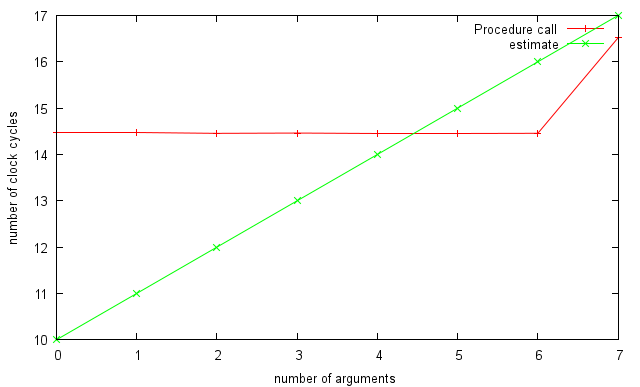
\includegraphics{procCallImage}
That's not much work and the total cost of a procedure call should be around 15
cycles. Each argument may increase the overhead of 1 of 2 cycles.
The result shows us that the base result for a procedure call is around 15
cycles and that each argument increase the cost by 1 or 2 cycles as excepted.

\subsubsection{System call overhead}
We choosed the getpid() system call to test the overhead for a minimal system
call as it's supposed the least expensive system call.
System call are excepted to be more expensive than simple procedure call as they
produce a context switch.
The result shows that a system call takes around 800 clock cycles to complete.

\subsubsection{Task creation time}
For testing the overhead of creating a new process, we simply called fork(). It turned out that it takes about 750,000 clock cycles for creating it without caching and less than 500,000 with caching.While for the overhead of creating a new thread, we simply called pthread\_creat(). It turned out that it takes about 2000,000 clock cycles for creating it without caching and less than 80,000 with caching.
The fact thread creation without caching is taking way longer time than the one for process creation doesn't really make sense to us right now, and we will look into that later as the project goes. But considering that thread creation does't envolve memory alloction, the average case for thread creation is generally faster then the one for process creation.


\subsubsection{Context switch time}
We measured the context switching overhead for both processes and threads. The way we define context switching is by creating a child process/thread and make the child do some task and return back to the parent. The overhead of such context switching is going to be the time start from the creation of the child to the time execution gets back to the parent process/thread excluding the time for child to execute. We only tested the context switching within 2 different processes.
//***TODO actual result

\subsection{Random Access Memory}

\subsubsection{RAM access time}
We measured the back-to-back-load RAM access latency, because it is well accepted by most software developers and system researchers. The way we measure the RAM access latency is making the program iterating a array of specific size for bunch of times and averaging it to eliminate the noise. The size of the array we used are larger than 256KB, which is larger than the total amount of L1 cache and L2 cache. We did multiple number of tests on iterating the first k element of the array, so that certain part of the data will be cached into L1 cache or L2 cache.
We expected to see the RAM access time increases as it goes from L1, L2 to main memory. Basically saying there would be a significant difference among the following three cases: 
1. iteration of the first 32KB data or less (fit into L1 cache)
2. iteration of the first 288KB data or less (fit into L1+L2 cache)
3. iteration of all the whole array(doesn’t fit into caches).
The result we got from our measurement shown that //TODO actual result






\subsubsection{RAM bandwidth}

We used an array with size 16MB, so that it is larger than the cache size (6MB including fancy L3 cache). At the same time, it still fits into the main memory. We iterated through the list and do both read and write. We did read by just doing a[i]+0 and write by doing a[i] = a[i]+1. We would expect read is faster than write operation, because the system need to make sure the data is actually write to the memory after performed the write operation. While there is no such issue for read operation.





\subsubsection{Page fault service time}

In order to manually create a page fault situation, we used two really large array which as the same size as main memory. Then we are going to iterate through the first array, basically means put it into main memory first. Afterwards, we iterate through the second array so that the first array will be totally paged out to hardddisk after that. The page fault service time is going to be the time it takes for us to get the value of element from first array at this point.This forces the page to swap gives us the right page fault service time. 


%\clearpage
\phantomsection
\addcontentsline{toc}{chapter}{Bibliographie}
\begin{thebibliography}{99}
\bibitem{intel-i5-2500} \url{http://ark.intel.com/products/52209}
\bibitem{dq670w-motherboard} \url{http://www.intel.com/content/www/us/en/motherboards/desktop-motherboards/desktop-board-dq67ow.html}
\bibitem{q67-chipset} \url{http://www.intel.com/content/www/us/en/chipsets/mainstream-chipsets/q67-express-chipset.html}
\bibitem{p7k500} \url{http://www.hitachigst.com/tech/techlib.nsf/products/Deskstar_P7K500}
\bibitem{7K1000.C} \url{http://www.hitachigst.com/internal-drives/desktop/deskstar/deskstar-7k1000c}
\bibitem{intel-archi-opti-intel64} Intel® 64 and IA-32 Architectures Optimization Reference Manual \url{http://www.intel.com/Assets/en_US/PDF/manual/248966.pdf}
\bibitem{zfs-evil-tuning} Guide on tuning ZFS
\url{http://www.solarisinternals.com/wiki/index.php/ZFS\_Evil\_Tuning\_Guide#Limiting\_the\_ARC\_Cache}
\bibitem{zfs-arc-max} ZFS tuning official documentation
\url{http://docs.oracle.com/cd/E23824\_01/html/821-1450/chapter2-2.html#gjhec}
\bibitem{intel-xeon-3565} \url{http://ark.intel.com/products/39721}
\end{thebibliography}


\end{document}
